In order to understand the requirements for the underlying server PC, a validation system based on Intel(R) Xeon(R) CPU E5-1650 v2 
@ 3.5 GHz with six cores is being used to perform tests of the PC based RoIB. 
The goal is to perform software based fragment assembly at a rate of 100 kHz over 12 channels for a typical 
fragment size of 400 bytes. The current system offers flexibility in terms of the fragment size allowed which was not the case in the 
VMEbus based RoIB. The initial tests were performed with a standalone application that implements a minimal interface for event building. 
Once the system was validated, the relevant code modules were integrated into an HLTSV process running within the full ATLAS TDAQ 
software suite with appropriately scaled test hardware to represent the remaining elements of the system.

\subsection{Standalone Tests}\label{sec:perf_alone}

The goal was to test input/output bandwidth limitations of the RobinNP and the rate of event building. Initial performance testing used 
a standalone RobinNP application and an external source that emulates the L1 trigger data 
in the form of 32-bit word fragments with 12 channels. In this test, the host PC was running the assembly routine with a single threaded application.  Figure \ref{fig:fig:roib_summary} shows the input rate without 
event building as a function of fragment size. For 400 byte fragments the input rate to the RobinNP is 215 kHz. 
The same figure 
shows the event building rate which is 150 kHz. This performance shows that the event building 
at the required rate of 100 kHz with 12 channels is achievable in a standalone application.  


%% \begin{figure}[tbp] % figures (and tables) should go top or bottom of
%%   % the page where they are first cited or in
%%   % subsequent pages
%%   \centering
%%   \includegraphics[width=.7\textwidth]{fig:roib_summary.pdf}
%%   \caption{Rate as a function of the fragment size (in bytes) with external source that emulates the L1 trigger input. 
%%     The rates shown are for the input rate to the RobinNP without event building (EB) (triangle), rate with EB (circle), and 
%%     for comparison, the current VMEbus RoIB rate is also shown (square).  }
%%   \label{fig:fig:roib_summary}
%% \end{figure}


\subsection{Full System Tests}\label{sec:perf_tdaq}

Since the HLTSV is performing tasks other than the event building, there is overhead associated with additional operations 
that reduces the performance. For this reason, we use the full ATLAS TDAQ software in a test environment that emulates the major components of the ATLAS data acquisition system shown in Figure \ref{fig:atlas_tdaq}. The setup includes an emulated input from L1 trigger sources, 
the HLTSV and other PCs to simulate the HLT computing farm, and the ROS that buffers the full event data. 
 In this test setup, an external source sends data that emulates L1 RoIs via 12 links connected to the 
RobinNP hosted by the HLTSV. When the HLTSV requests a built RoI event, the software RoIB plug-in provides the RoI event which will be used 
to seed requests for the event data to be processed.
 Figure \ref{fig:partition} shows an event building rate of 110 kHz measured with 400 byte fragments with the HLTSV application in a setup close to the ATLAS TDAQ system. 

\begin{figure}[tbp] % figures (and tables) should go top or bottom of
                    % the page where they are first cited or in
                    % subsequent pages
\centering
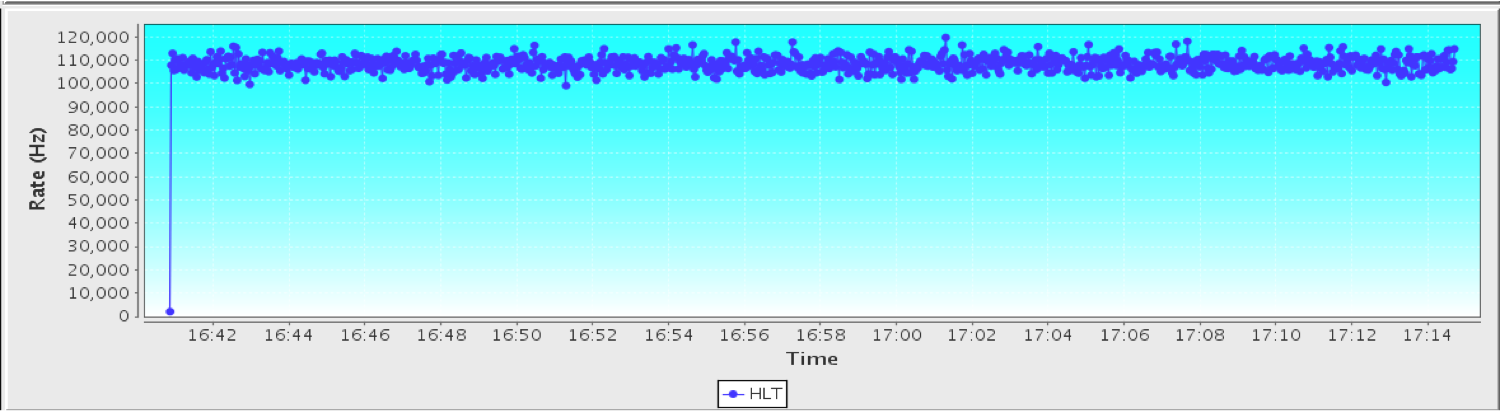
\includegraphics[width=.98\textwidth]{12ch.png}
\caption{Screenshot of a monitoring tool which shows the HLTSV processing rate using the ATLAS TDAQ software .}
\label{fig:partition}
\end{figure}

